%%%%%%%%%%%%%%%%%%%%%%%%%%%%%%%%%%%%%%%%%%%%%%%%%%%%%%
% A Beamer template for University of Wollongong     %
% Based on THU beamer theme                          %
% Author: Qiuyu Lu                                   %
% Date: July 2024                                    %
% LPPL Licensed.                                     %
%%%%%%%%%%%%%%%%%%%%%%%%%%%%%%%%%%%%%%%%%%%%%%%%%%%%%%

\documentclass[aspectratio=169]{beamer}
\usepackage[scaled=0.9]{helvet}
\usepackage{courier}
\usepackage[T1]{fontenc}
\usepackage{hyperref}
\usepackage{latexsym,amsmath,xcolor,multicol,booktabs,calligra}
\usepackage{graphicx,pstricks,listings,stackengine}


\usepackage{inputenx} 
\usetheme{Madrid}
\usecolortheme{seahorse}

\usepackage{tikz}
% Configuration de TikZ pour la mise en évidence
\tikzset{
    highlight on/.style={
        alt={#1{fill=red!80!black, color=red!80!black}{fill=gray!30!white, color=gray!30!white}},
    },
}

\author{EL HASSANI Nabil}
\title{Design pattern}
\subtitle{Introduction aux design patterns}
\institute{
    Efrei \\
    Université Paris Panthéon-Assas
    }
    \date{\small \today}
\usepackage{UoWstyle}

% defs
\def\cmd#1{\texttt{\color{red}\footnotesize $\backslash$#1}}
\def\env#1{\texttt{\color{blue}\footnotesize #1}}
\definecolor{deepblue}{rgb}{0,0,0.5}
\definecolor{deepred}{RGB}{153,0,0}
\definecolor{deepgreen}{rgb}{0,0.5,0}
\definecolor{halfgray}{gray}{0.55}

\lstset{
    basicstyle=\ttfamily\small,
    keywordstyle=\bfseries\color{deepblue},
    emphstyle=\ttfamily\color{deepred},    % Custom highlighting style
    stringstyle=\color{deepgreen},
    numbers=left,
    numberstyle=\small\color{halfgray},
    rulesepcolor=\color{red!20!green!20!blue!20},
    frame=shadowbox,
}

%\setbeameroption{show notes on second screen=left}
\titlegraphic{
\includegraphics[height=1.5cm]{pic/efrei_logo.png}}
%==========================================================
\begin{document}
%==========================================================
\begin{frame}
    \titlepage
\end{frame}

\begin{frame}
    \tableofcontents[hideallsubsections]
\end{frame}
\section{test}
\begin{frame}[t]
    \frametitle{Historique des Design Patterns}
    
    \begin{tikzpicture}[xscale=0.8, yscale=1.5, every node/.style={scale=0.9}]
        % Ligne principale de la timeline
        \draw[line width=1mm, -latex, red!50] (-0.2,0) -- (15,0);
        
        % Boucles sur les années avec animation (onslide pour l'affichage séquentiel)
        \foreach \X [evaluate=\X as \Y using int(\X-1970), count=\Z] in {1977, 1987, 1994, 1995, 2004, 2010} {
            \onslide<\Z->{% Affiche la section de la timeline au bon moment
                \draw[fill=red!80!black, color=red!80!black] (\Y-0.2,-0.5) -- (\Y+0.2,-0.5) -- (\Y,-0.1) -- cycle;
                \node[anchor=south, fill=white, rotate=45, anchor=south west, inner sep=0pt] at (\Y,0.2) {\X};
            }
        }
    \end{tikzpicture}
    
    % Liste des événements animés
    \begin{itemize}
        \item<1> \textbf{1977}: Christopher Alexander introduit l'idée de patrons dans l'architecture.
        \item<2> \textbf{1987}: Ward Cunningham et Kent Beck appliquent l'idée de *patterns* en génie logiciel.
        \item<3> \textbf{1994}: Publication du livre « *Design Patterns: Elements of Reusable Object-Oriented Software* » par le Gang of Four.
        \item<4> \textbf{1995}: Les *design patterns* deviennent populaires avec Java et les langages orientés objet.
        \item<5> \textbf{2004}: Première conférence internationale sur les *patterns* (PLOP).
        \item<6> \textbf{2010}: Adoption massive des *design patterns* dans le développement Agile et les pratiques DevOps.
    \end{itemize}
    
    \end{frame}
    
%==========================================================
\section{Introduction}
    \subsection{Objectif du Cours}
        \begin{frame}{Objectif du Cours}
            \begin{itemize}
                \item<1-> \textbf{But principal :} Comprendre les concepts fondamentaux des \textbf{Design Patterns} et savoir comment les appliquer dans la conception orientée objet.
                \item<2-> \textbf{Focus sur :} 
                \begin{itemize}
                    \item L'importance des Design Patterns pour améliorer la flexibilité, la réutilisabilité et la maintenabilité des logiciels.
                    \item L'apprentissage des patterns les plus courants, tels que \textit{Singleton, Factory, Adapter, Observer, Strategy}.
                \end{itemize}                
                \item<3-> \textbf{À la fin du cours :} Vous serez capable de :
                \begin{itemize}
                    \item Développer la capacité à identifier le pattern approprié en fonction du contexte.
                    \item Maîtriser l'utilisation des design patterns pour résoudre des problèmes de conception.                    
                \end{itemize}
            \end{itemize}
            \only<4>{
            \begin{alertblock}{Note} {
                Tous les \textbf{Design Patterns} existants ne seront pas abordés dans ce cours. Nous nous concentrerons sur ceux qui sont les plus utilisés dans le développement moderne.
            }
            \end{alertblock}   
            }
        \end{frame}
    \subsection{Historique}
        \begin{frame}{Histoire des Design Patterns}
            \begin{itemize}
                \item \textbf{Années 1970} : Le concept de "patterns" a été introduit par \textbf{Christopher Alexander}, un architecte qui a formalisé l'idée de modèles réutilisables en architecture.
                \item \textbf{Années 1980} : Les premières applications de ces concepts dans le développement logiciel ont vu le jour avec la programmation orientée objet.
                \item \textbf{1994} : Publication du livre fondateur \textit{"Design Patterns: Elements of Reusable Object-Oriented Software"} par les \textbf{Gang of Four} (GoF) :
                    \begin{itemize}
                        \item Erich Gamma
                        \item Richard Helm
                        \item Ralph Johnson
                        \item John Vlissides
                    \end{itemize}
                \item \textbf{Objectif} : Fournir des solutions réutilisables aux problèmes récurrents dans la conception de logiciels orientés objet.
                \item \textbf{Depuis les années 2000} : Les *Design Patterns* sont devenus un élément central de l'enseignement et de la pratique de la conception logicielle.
            \end{itemize}
        \end{frame}

\section{Design pattern}
    \subsection{Motivation}
        \begin{frame}{Pourquoi les Design Patterns ?}
            \textbf{Les Design Patterns} fournissent des solutions éprouvées à des problèmes de conception récurrents dans le développement orienté objet. Ils permettent une meilleure communication entre développeurs, facilitent la maintenabilité et l'évolution du code, et encouragent la réutilisation de solutions. Nous allons explorer les raisons clés d'utiliser les Design Patterns.
        \end{frame}

        \begin{frame}{1. Des solutions réutilisables aux problèmes récurrents}
            \begin{itemize}
                \item Les Design Patterns offrent des solutions standardisées aux problèmes rencontrés régulièrement dans différents projets.
                \item \textbf{Exemple :} Le \textbf{Singleton} permet de s'assurer qu'une classe n'a qu'une seule instance (par exemple, une connexion unique à une base de données).
            \end{itemize}
        \end{frame}

        \begin{frame}{2. Amélioration de la communication}
            \begin{itemize}
                \item Les Design Patterns créent un vocabulaire commun entre développeurs.
                \item Lorsqu'un développeur mentionne un pattern (\textit{ex : Utilisons un Factory ici}), l'équipe comprend immédiatement l'intention de conception.
                \item Cela simplifie la collaboration et aide les nouveaux membres à s'intégrer plus rapidement.
            \end{itemize}
        \end{frame}

        \begin{frame}{3. Faciliter la maintenabilité et l’évolution du code}
            \begin{itemize}
                \item Les Design Patterns aident à concevoir des systèmes flexibles et modulaires, facilitant l’ajout de nouvelles fonctionnalités sans devoir réécrire le code.
                \item \textbf{Exemple :} Le \textbf{Observer} permet de réagir aux changements d'état sans affecter d'autres parties du système.
            \end{itemize}
        \end{frame}

        \begin{frame}{4. Réutilisation de l’expérience plutôt que du code}
            \begin{itemize}
                \item Les Design Patterns permettent de réutiliser des solutions et des stratégies déjà éprouvées dans d'autres projets.
                \item Cela améliore non seulement la qualité des logiciels, mais aussi les compétences des développeurs.
                \item \textbf{Idée clé :} Avec les patterns, vous réutilisez de l’expérience, pas seulement du code.
            \end{itemize}
        \end{frame}

        \begin{frame}{5. Renforcer la flexibilité et la modularité}
            \begin{itemize}
                \item Les Design Patterns encouragent la séparation des préoccupations et la modularité du code.
                \item Cela permet de changer des fonctionnalités sans affecter le reste du système.
                \item \textbf{Exemple :} Le \textbf{Strategy} permet de changer d'algorithme à l'exécution sans modifier le cœur du programme.
            \end{itemize}
        \end{frame}

        \begin{frame}{6. Quand utiliser les Design Patterns ?}
            \begin{itemize}
                \item Utilisez les Design Patterns pour des problèmes récurrents avec des solutions standardisées.
                \item Évitez de les surutiliser dans des projets simples, où des solutions spécifiques peuvent suffire.
                \item \textbf{Conseil :} Soyez attentifs aux situations où un pattern améliore réellement la structure et la maintenabilité du code.
            \end{itemize}
        \end{frame}

        \begin{frame}{Conclusion}
        \begin{itemize}
            \item Les Design Patterns apportent des solutions robustes et éprouvées.
            \item Ils facilitent la communication, la maintenabilité et l'évolutivité des systèmes logiciels.
            \item Leur utilisation doit être réfléchie, pour éviter la complexité inutile.
            \item En les adoptant, vous améliorez la qualité de vos conceptions tout en réduisant la complexité et en facilitant l'évolution du code à long terme.
        \end{itemize}
        \end{frame}
    \subsection{Catégories}
        \begin{frame}{Catégories}
            \begin{columns}
                \begin{column}{0.5\textwidth}
                    \onslide<1>{  
                        \centering
                        \par Il existe trois grandes catégories de design patterns
                    }
                    \begin{itemize}
                        \item<2-> \textbf{Créationnels :} Concernent la manière dont les objets sont créés.             
                        \item<3-> \textbf{Structurels :} Traitent de l'organisation des classes et des objets, ainsi que de leurs relations.               
                        \item<4-> \textbf{Comportementaux :} Concernent l'interaction et la communication entre objets.
                    \end{itemize}
                \end{column}
                \begin{column}{0.5\textwidth}
                    \only<1>{
                        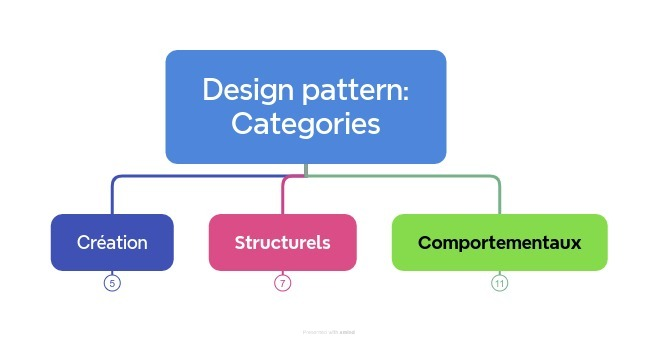
\includegraphics[width=\textwidth]{pic/dep_categorie_1.jpg}
                    }
                    \only<2>{
                        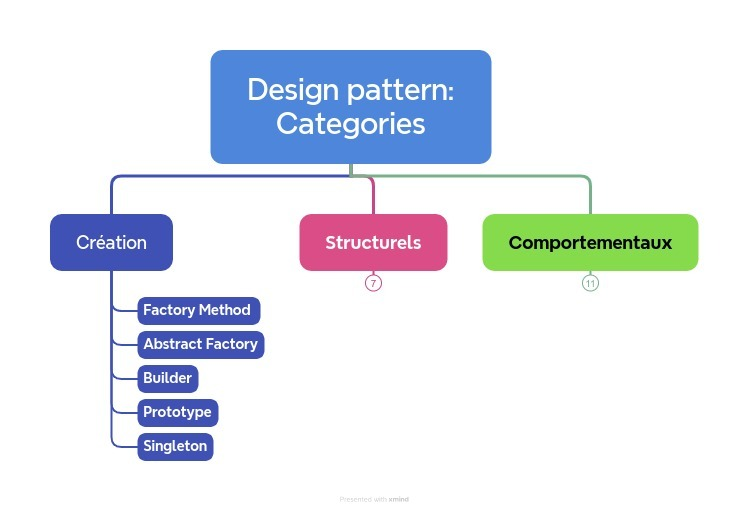
\includegraphics[width=\textwidth]{pic/dep_categorie_2.jpg}
                    }
                    \only<3>{
                        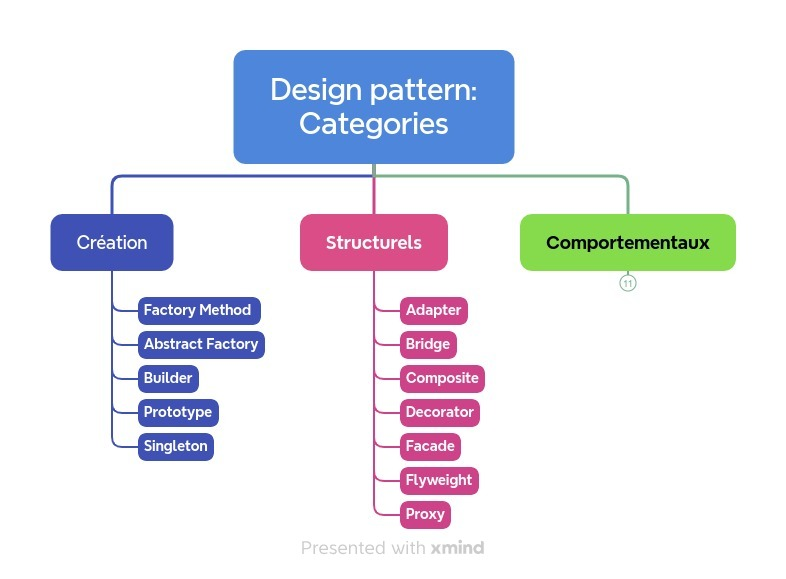
\includegraphics[width=\textwidth]{pic/dep_categorie_3.jpg}
                    }
                    \only<4>{
                        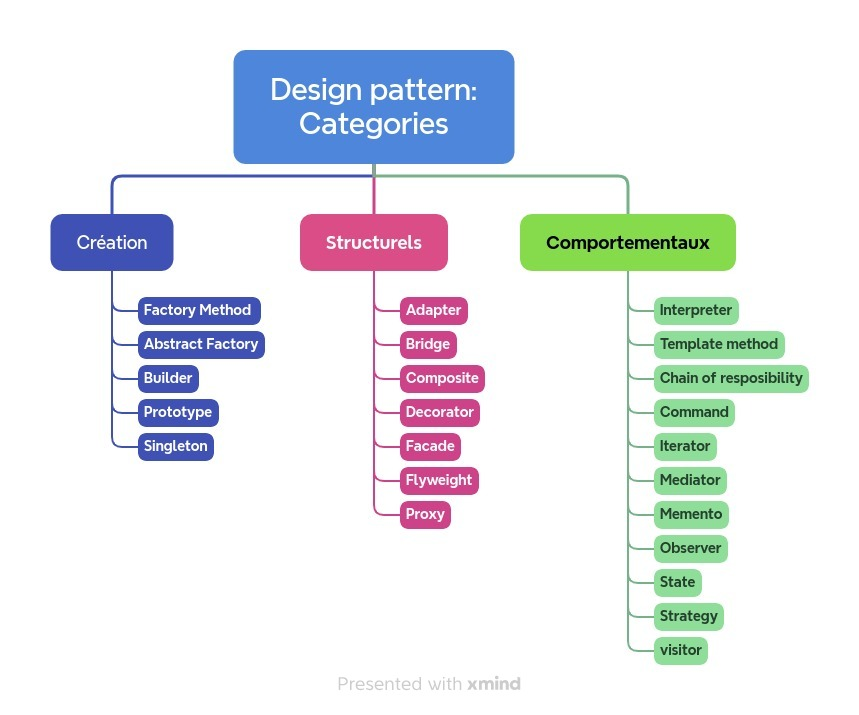
\includegraphics[width=\textwidth]{pic/dep_categorie_4.jpg}
                    }
                \end{column}
            \end{columns}
        \end{frame}


\section{Rappel des fondamentaux OO}
    \begin{frame}{Pourquoi l'approche POO (Programmation Orientée Objet)}
        \begin{itemize}
            \item \textbf{Modularité :} Favorise la division du code en modules réutilisables (classes et objets).
            \item \textbf{Réutilisabilité :} Encourage la réutilisation du code grâce à l'héritage et à la composition.
            \item \textbf{Facilité de maintenance :} Le code orienté objet est plus facile à comprendre, tester, et modifier.
            \item \textbf{Correspond à la réalité :} Permet de modéliser des objets du monde réel de manière plus naturelle en représentant des entités avec des propriétés et des comportements.
        \end{itemize}
    \end{frame}

    \begin{frame}{Rappel : Principes de la POO (Programmation Orientée Objet)}
        \begin{itemize}
            \item \textbf{Encapsulation :} Les données (attributs) et les comportements (méthodes) sont regroupés dans des objets. Les détails internes sont cachés et protégés.
            \item \textbf{Héritage :} Les classes peuvent hériter des attributs et méthodes d'une autre classe pour éviter la duplication et faciliter la réutilisation du code.
            \item \textbf{Polymorphisme :} Permet à une méthode d’avoir plusieurs implémentations, ce qui favorise la flexibilité dans le code.
            \item \textbf{Abstraction :} Les objets représentent des concepts abstraits qui modélisent des éléments du monde réel, simplifiant ainsi la conception et la compréhension du code.
        \end{itemize}
    \end{frame}

    \begin{frame}{Comparaison : Héritage vs Composition}
        \begin{itemize}
            \item \textbf{Héritage :}
            \begin{itemize}
                \item Relation "est-un" : La sous-classe hérite des propriétés et comportements de la classe parent.
                \item Favorise la réutilisation de code mais peut entraîner une dépendance forte entre les classes.
                \item \textit{Exemple :} Un \textbf{Chien} hérite de la classe \textbf{Animal}.
            \end{itemize}

            \item \textbf{Composition :}
            \begin{itemize}
                \item Relation "a-un" : Une classe est composée d'autres classes.
                \item Favorise une conception plus flexible, car les composants peuvent être remplacés ou modifiés plus facilement.
                \item \textit{Exemple :} Une \textbf{Voiture} est composée d'un \textbf{Moteur}, \textbf{Roues}, etc.
            \end{itemize}
            
            \item \textbf{Conclusion :} La composition est souvent préférée à l’héritage, car elle permet une meilleure flexibilité et évolutivité, tout en évitant les problèmes liés à une hiérarchie d'héritage rigide.
        \end{itemize}
    \end{frame}

\section{References}
    \begin{frame}[allowframebreaks]
        {
            \tiny
            \bibliographystyle{alpha}
            \bibliography{ref}
        }
    \end{frame}


    \begin{frame}
        \begin{center}
            {\Huge\calligra Merci}
        \end{center}
    \end{frame}

\end{document}